%%%%%%%%%%%%%%%%%%%%%%%%%%%%%%%%%%%%%%%%%%%%%%%%%%%%%%%%
%%%%%%%%%%%%%%%%%%%%%%%%%%%%%%%%%%%%%%%%%%%%%%%%%%%%%%%%
%%%%%%%%%%%%%%%%%%%%%%%%%%%%%%%%%%%%%%%%%%%%%%%%%%%%%%%%
\chapter{General Machine Learning Concepts}
\label{ml:general}

%%%%%%%%%%%%%%%%%%%%%%%%%%%%%%%%%%%%%%%%%%%%%%%%%%%%%%%%
%%%%%%%%%%%%%%%%%%%%%%%%%%%%%%%%%%%%%%%%%%%%%%%%%%%%%%%%
\section{Evaluating Performance}
\label{ml:general:eval}

%%%%%%%%%%%%%%%%%%%%%%%%%%%%%%%%%%%%%%%%%%%%%%%%%%%%%%%%
\subsection{Confusion Matrix}
\label{ml:general:eval:cm}

The confusion matrix is a simple table of the number of actual, or truth, class instances
versus the number of a model's predicted class instances.
A two class example is provided in \cref{table:CM}.
Multi-class confusion matrices are straight forward extensions,
with correctly classified instances appearing along the diagonal.

\begin{table}[H]
  \centering
  \begin{tabular}{c | c | c | c |}
  \multicolumn{2}{c}{} & \multicolumn{2}{c}{\textbf{Actual}} \\ \cline{3-4}
  \multicolumn{1}{c}{} & & Positive & Negative \\ \cline{2-4}
  \multirow{4}{*}{\rotatebox{90}{\textbf{Predicted}}} & \multirow{2}{*}{Positive} & \multirow{2}{*}{TP} & FP \\[-8pt]
   & & & (Type I) \\ \cline{2-4}
   & \multirow{2}{*}{Negative} & FN & \multirow{2}{*}{TN} \\[-8pt]
   & & (Type II) & \\ \cline{2-4}
  \end{tabular}
  \caption{Two class confusion matrix.}
  \label{table:CM}
\end{table}

%%%%%%%%%%%%%%%%%%%%%%%%%%%%%%%%%%%%%%%%%%%%%%%%%%%%%%%%
\subsection{TPR \& TNR -- Sensitivity \& Specificity}
\label{ml:general:eval:TPR_TNR}

The true positive rate (TPR) and true negative rate (TNR) are
relatively straight forward to compute and understand, along with their complements,
the false negative rate (FNR), \ie miss rate, and false positive rate (FPR), \ie fall-out.
Here the denominators are the number of true class members.

\begin{enumerate}[noitemsep]
\item True positive rate (TPR), \ie sensitivity, recall, hit rate:
\begin{equation} \label{eq:TPR}
\text{TPR} = \frac{\text{TP}}{\text{P}} = \frac{\text{TP}}{\text{TP}+\text{FN}} = 1 - \text{FNR} = P\left(\hat{+} \mid + \right)
\end{equation}

\item True negative rate (TNR), \ie specificity, selectivity:
\begin{equation} \label{eq:TNR}
\text{TNR} = \frac{\text{TN}}{\text{N}} = \frac{\text{TN}}{\text{TN}+\text{FP}} = 1 - \text{FPR} = P\left(\hat{-} \mid - \right)
\end{equation}
\end{enumerate}

%%%%%%%%%%%%%%%%%%%%%%%%%%%%%%%%%%%%%%%%%%%%%%%%%%%%%%%%
\subsection{PPV (Precision) \& NPV}
\label{ml:general:eval:PPV_NPV}

The positive predictive value (PPV), more commonly known as precision, and negative predictive value (NPV)
are related metrics, but with predicted class members in the denominators.
Their complements are the false discovery rate (FDR) and false omission rate (FOR).
It is helpful to look at these metrics graphically, as in \cref{fig:graphical_CM_quantities}.

\begin{enumerate}[noitemsep]
\item Positive predictive value (PPV), \ie precision:
\begin{equation} \label{eq:PPV}
\text{PPV} = \frac{\text{TP}}{\hat{\text{P}}} = \frac{\text{TP}}{\text{TP}+\text{FP}} = 1 - \text{FDR} = P\left(+ \mid \hat{+} \right)
\end{equation}

\item Negative predictive value (NPV):
\begin{equation} \label{eq:NPV}
\text{NPV} = \frac{\text{TN}}{\hat{\text{N}}} = \frac{\text{TN}}{\text{TN}+\text{FN}} = 1 - \text{FOR} = P\left(- \mid \hat{-} \right)
\end{equation}
\end{enumerate}

\begin{figure}[H]
\centering
  \begin{subfigure}[c]{0.48\textwidth}\centering
  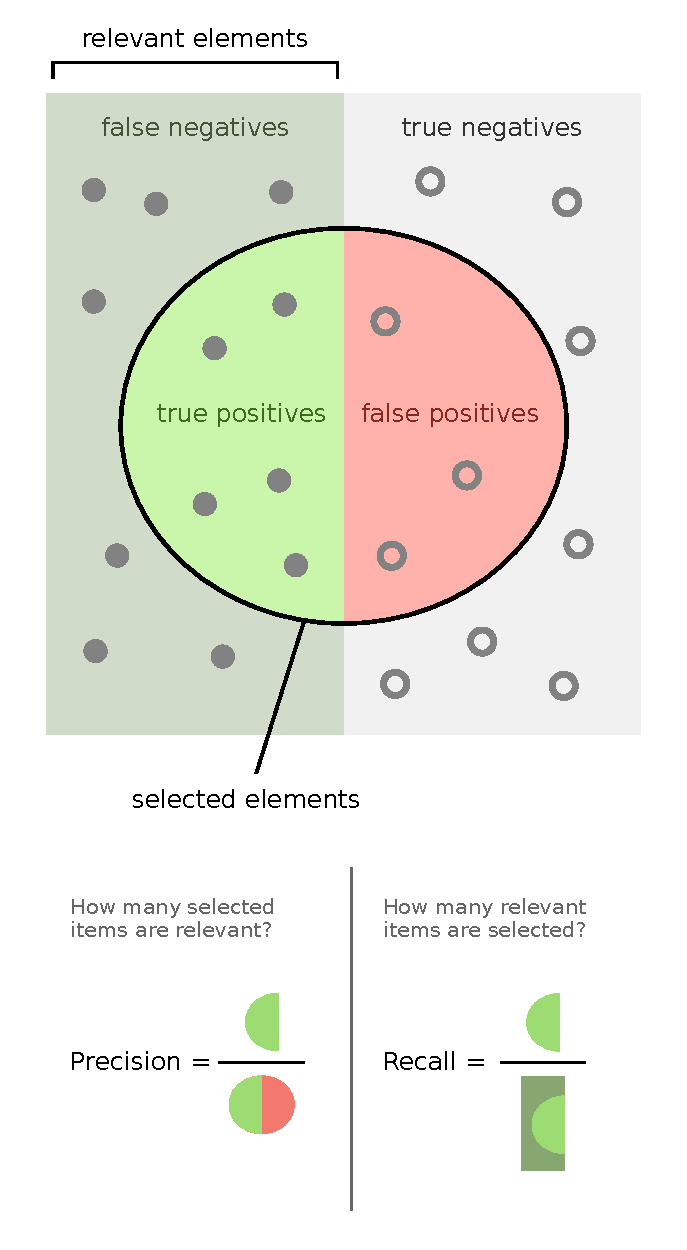
\includegraphics[width=\textwidth]{figures/ml/precision_recall}
  \caption{Precision \& Recall}
  \label{fig:graphical_CM_quantities:precision_recall}
  \end{subfigure}
  ~
  \begin{subfigure}[c]{0.48\textwidth}\centering
  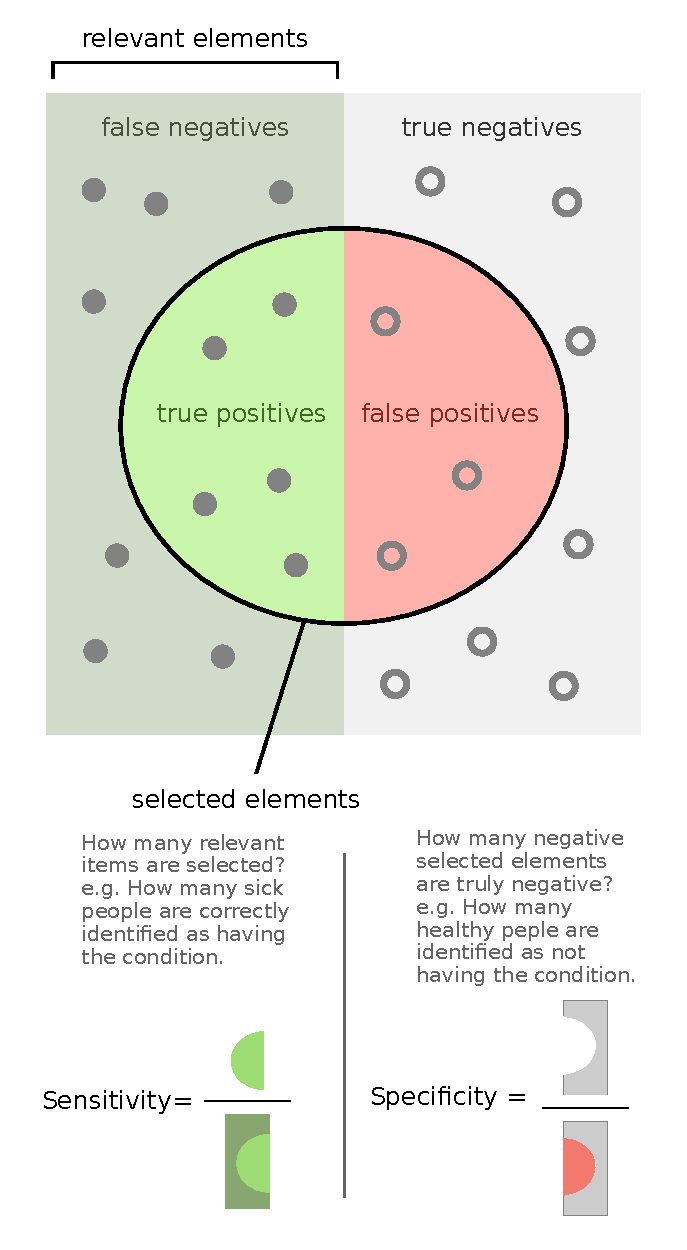
\includegraphics[width=\textwidth]{figures/ml/sensitivity_and_specificity}
  \caption{Sensitivity \& Specificity}
  \label{fig:graphical_CM_quantities:sensitivity_specificity}
  \end{subfigure}
\caption{
Graphical representation of
precision versus recall (sensitivity), by \href{https://commons.wikimedia.org/wiki/File:Precisionrecall.svg}{Walber},
and
sensitivity (recall) versus specificity, by \href{http://en.wikipedia.org/wiki/File:Sensitivity_and_specificity.svg}{FeanDoe}.
}
\label{fig:graphical_CM_quantities}
\end{figure}

%%%%%%%%%%%%%%%%%%%%%%%%%%%%%%%%%%%%%%%%%%%%%%%%%%%%%%%%
\subsection{Other Scores}
\label{ml:general:eval:other_scores}

The accuracy (ACC), the proportion of correct predictions, is a natural metric for measuring a classifiers performance.
Various F-scores, such as $F_{1}$ and $F_{\beta}$, combine precision and recall into one metric\footnote{Note that $F_{\beta}$ does not depend on TN at all, a potential shortcoming.}.
$F_{1}$ balances precision and recall equally, and is their harmonic mean,
while $F_{\beta}$ uses $\beta$ to assign different weights to each\footnote{$F_{2}$ weights recall over precision, $F_{0.5}$ weights precision over recall.}.

\begin{enumerate}[noitemsep]
\item Accuracy (ACC):
\begin{equation} \label{eq:ACC}
\text{ACC} = \frac{\text{TP}+\text{TN}}{\text{P}+\text{N}} = \frac{\text{TP}+\text{TN}}{\text{TP}+\text{TN}+\text{FP}+\text{FN}}
\end{equation}

\item $F_{1}$ ($F_{1}=1$ is best, $F_{1}=0$ is worst):
\begin{equation} \label{eq:F1}
F_{1} = \left(\frac{\text{precision}^{-1}+\text{recall}^{-1}}{2}\right)^{-1} = 2\,\,\frac{\text{precision} \times \text{recall}}{\text{precision} + \text{recall}}
\end{equation}

\item $F_{\beta}$ (Larger $\beta$ weights recall over precision):
\begin{equation} \label{eq:Fbeta}
F_{\beta} = \left(1+\beta^{2}\right) \frac{\text{precision} \times \text{recall}}{\beta^{2}\,\text{precision} + \text{recall}} =
\frac{\left(1+\beta^{2}\right) \text{TP}}{\left(1+\beta^{2}\right) \text{TP} + \beta^{2}\,\text{FN} + \text{FP}}
\end{equation}
\end{enumerate}

\clearpage% TODo hard coded
%%%%%%%%%%%%%%%%%%%%%%%%%%%%%%%%%%%%%%%%%%%%%%%%%%%%%%%%
%%%%%%%%%%%%%%%%%%%%%%%%%%%%%%%%%%%%%%%%%%%%%%%%%%%%%%%%
\section{Bias-Variance Tradeoff}
\label{ml:general:bias_variance_tradeoff}

\begin{enumerate}[noitemsep]
\item Bias: Errors due to a model not learning about relationships between features in the training data, \ie underfitting. Caused by invalid relationships present in the model.
\item Variance: Errors due to an overly complex model failing to generalize beyond the training data, \ie overfitting. Caused by sensitivity to small fluctuations in the training data.
\end{enumerate}

\begin{figure}[H]
  \centering
  \savebox{\largestimage}{
    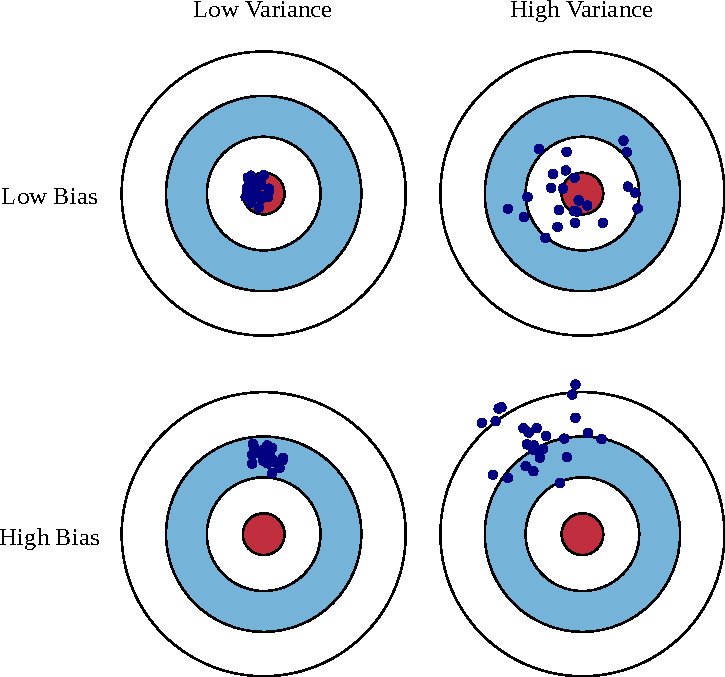
\includegraphics[width=0.47\textwidth]{figures/ml/bias_variance_tradeoff}
  }% Store largest image in a box

  \begin{subfigure}[b]{0.48\textwidth}\centering
    \usebox{\largestimage}
    \vspace{0.01cm}
  \caption{Direct Comparison}
  \label{fig:ml:bias_variance_tradeoff:direct}
  \end{subfigure}
  ~
  \begin{subfigure}[b]{\wd\largestimage}\centering
    \raisebox{\dimexpr.5\ht\largestimage-.5\height}{% Adjust vertical height of smaller image
      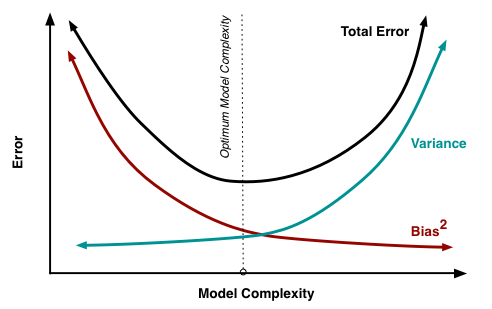
\includegraphics[width=\textwidth]{figures/ml/bias_variance_error_tradeoff.png}}
  \caption{Error Components (Test Set)}
  \label{fig:ml:bias_variance_tradeoff:error}
  \end{subfigure}
\caption{
Illustrations of the bias-variance tradeoff,
by \href{http://scott.fortmann-roe.com/docs/BiasVariance.html}{Scott Fortmann-Roe}.
\label{fig:ml:bias_variance_tradeoff}
}
\end{figure}

Every model makes a tradeoff between bias and variance,
which is roughly controlled by its level of complexity
as can be seen in \cref{fig:ml:bias_variance_tradeoff:error}.
\Cref{fig:additional:ml:general:early_stopping} shows this in practice,
as past a certain point of complexity the validation error grows
while the training error continues to decrease.

\subsubsection{Mean Square Error (MSE) Decomposition}
\label{ml:general:bias_variance_tradeoff:decop}

We can analytically decompose the mean square error (MSE) into explicit
bias, variance, and irreducable error components.
Let $y = f\left(\mathbf{x}\right) + \epsilon$ represent
the observed data, $y_{i}$, $\mathbf{x}_{i}$,
where $f\left(\mathbf{x}\right)$ is the true parent distribution\footnote{$\expval{f} = f$ is deterministic,
and acts as a constant as far as expectation values are concerned.} and
$\epsilon$ is random noise\footnote{This is the source of the irreducible error.
Since future data will still have $\epsilon$, the predictions can't be perfect
-- even when neglecting the model's own bias and variance.}\footnote{Later we'll need
$\sigma^{2} = \variance{\epsilon} = \expval{\epsilon^{2}} - \expval{\epsilon}^{2} = \expval{\epsilon^{2}}$.} having
$\expval{\epsilon} = 0$, $\variance{\epsilon} = \sigma^{2}$.
Representing the trained model\footnote{Note
that $\cov{\epsilon}{\hat{f}} = 0 \Rightarrow \expval{\epsilon \hat{f}} = \expval{\epsilon} \expval{\hat{f}}$.} as
$\hat{f}\left(\mathbf{x}\right)$, we expand the MSE:

\begin{subequations} \label{eq:bias_variance_tradeoff:decop}
\begin{align}
\text{MSE} &= \expval{\left(y-\hat{f}\right)^{2}} \\
&= \expval{\left(f + \epsilon - \hat{f} + \big[\expval{\hat{f}}-\expval{\hat{f}}\big]\right)^{2}}\,, \\
&= \expval{\left(\big[f - \expval{\hat{f}}\big] + \epsilon - \big[\hat{f} - \expval{\hat{f}}\big]\right)^{2}}\,, \\
&= \expval{\left(f-\expval{\hat{f}}\right)^{2}}
+\expval{\epsilon^{2}}
+\expval{\left(\hat{f}-\expval{\hat{f}}\right)^{2}}
+2\expval{\left(f-\expval{\hat{f}}\right)\epsilon} \\
&\hphantom{=}-2\expval{\epsilon\left(\hat{f}-\expval{\hat{f}}\right)}
-2\expval{\left(f-\expval{\hat{f}}\right)\left(\hat{f}-\expval{\hat{f}}\right)}\,, \\
&= \left(-1\right)^{2}\left(\expval{\hat{f}}-f\right)^{2} +\sigma^{2} + \variance{\hat{f}}
+2\left(f-\expval{\hat{f}}\right)\cancelto{0}{\expval{\epsilon}} \\
&\hphantom{=}-2\cancelto{0}{\expval{\epsilon}}\left(\expval{\hat{f}}-\expval{\hat{f}}\right)
-2\left(f-\expval{\hat{f}}\right)\cancelto{0}{\left(\expval{\hat{f}}-\expval{\hat{f}}\right)}\,, \\
&= \left(\bias{\hat{f}}\right)^{2} + \variance{\hat{f}} + \sigma^{2}\,.
\end{align}
\end{subequations}

\clearpage% TODo hard coded
%%%%%%%%%%%%%%%%%%%%%%%%%%%%%%%%%%%%%%%%%%%%%%%%%%%%%%%%
%%%%%%%%%%%%%%%%%%%%%%%%%%%%%%%%%%%%%%%%%%%%%%%%%%%%%%%%
\section{Regularization}
\label{ml:general:reg}

Regularization is a method for controlling the variance (overfitting)
of a model by putting constraints on the size of its parameters.
In terms of \cref{ml:general:bias_variance_tradeoff}, regularization forces the model's
bias to grow on the training set in order to lower the variance on future data.
The two main types of regularization are shown in \cref{eq:L1_L2}
and depend on different powers of the norm\footnote{In
the case of OLS linear regression the constant intercept term $\beta_{0}$ is not included in $\norm{\bm{\beta}}$.} of the model parameters $\bm{\beta}$.
In order to treat all features equally, normalization must be used before applying regularization.
A hyperparameter $\lambda$ is included to tune the amount of regularization applied in the objective function,
$S\left(\bm{\beta}\right) = L + \Omega$.
As $\lambda$ is increased, it decreases the size the model's coefficients, and thereby its variance (overfitting),
up to a point when the model is unable to adequately train on the available data and the bias (underfitting) begins to grow.

\begin{subequations} \label{eq:L1_L2}
\begin{align}
\Omega_{\text{L1}}\left(\bm{\beta}\right) &= \lambda \norm{\bm{\beta}}\hphantom{^{1}}
= \lambda \sum_{j=1}^{n} \, \abs{\beta_{j}}\,, \label{eq:L1} \\
\Omega_{\text{L2}}\left(\bm{\beta}\right) &= \lambda \norm{\bm{\beta}}^{2}
= \lambda \sum_{j=1}^{n} \,\, \beta_{j}^{2}\,. \label{eq:L2}
\end{align}
\end{subequations}

For a particular value of $\lambda$, the effect of L1 and L2 regularization\footnote{Here
$q$ is being used as the power of $\norm{\bm{\beta}}$. For L1 (L2), $q=1$ ($q=2$).} is
to constrain $\norm{\bm{\beta}}^{q} \leq t\left(\lambda\right)$ for some $t\left(\lambda\right)$.
As can be seen in \cref{fig:ml:l1l2} the L1 norm constrains $\bm{\beta}$ to lie within a hypercube,
while the L2 constraint is a hypersphere.

\begin{figure}[H]
  \centering
  \begin{subfigure}[b]{0.48\textwidth}\centering
      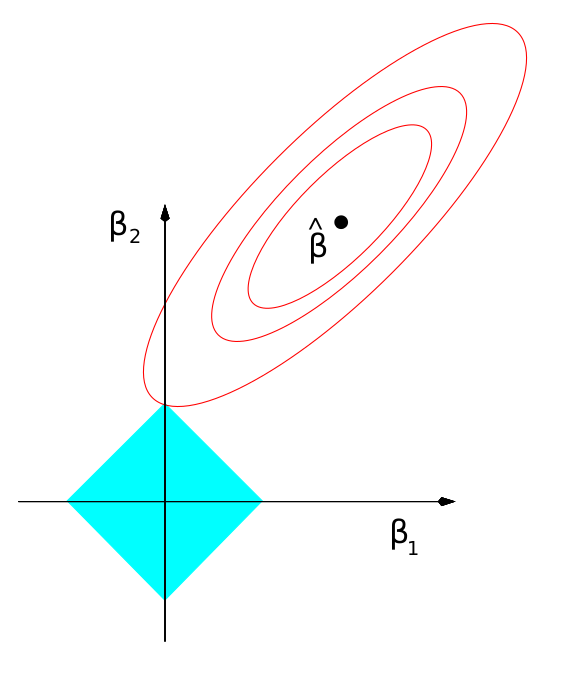
\includegraphics[width=\textwidth]{figures/ml/l1}
  \caption{L1}
  \label{fig:ml:l1l2:l1}
  \end{subfigure}
  ~
  \begin{subfigure}[b]{0.48\textwidth}\centering
      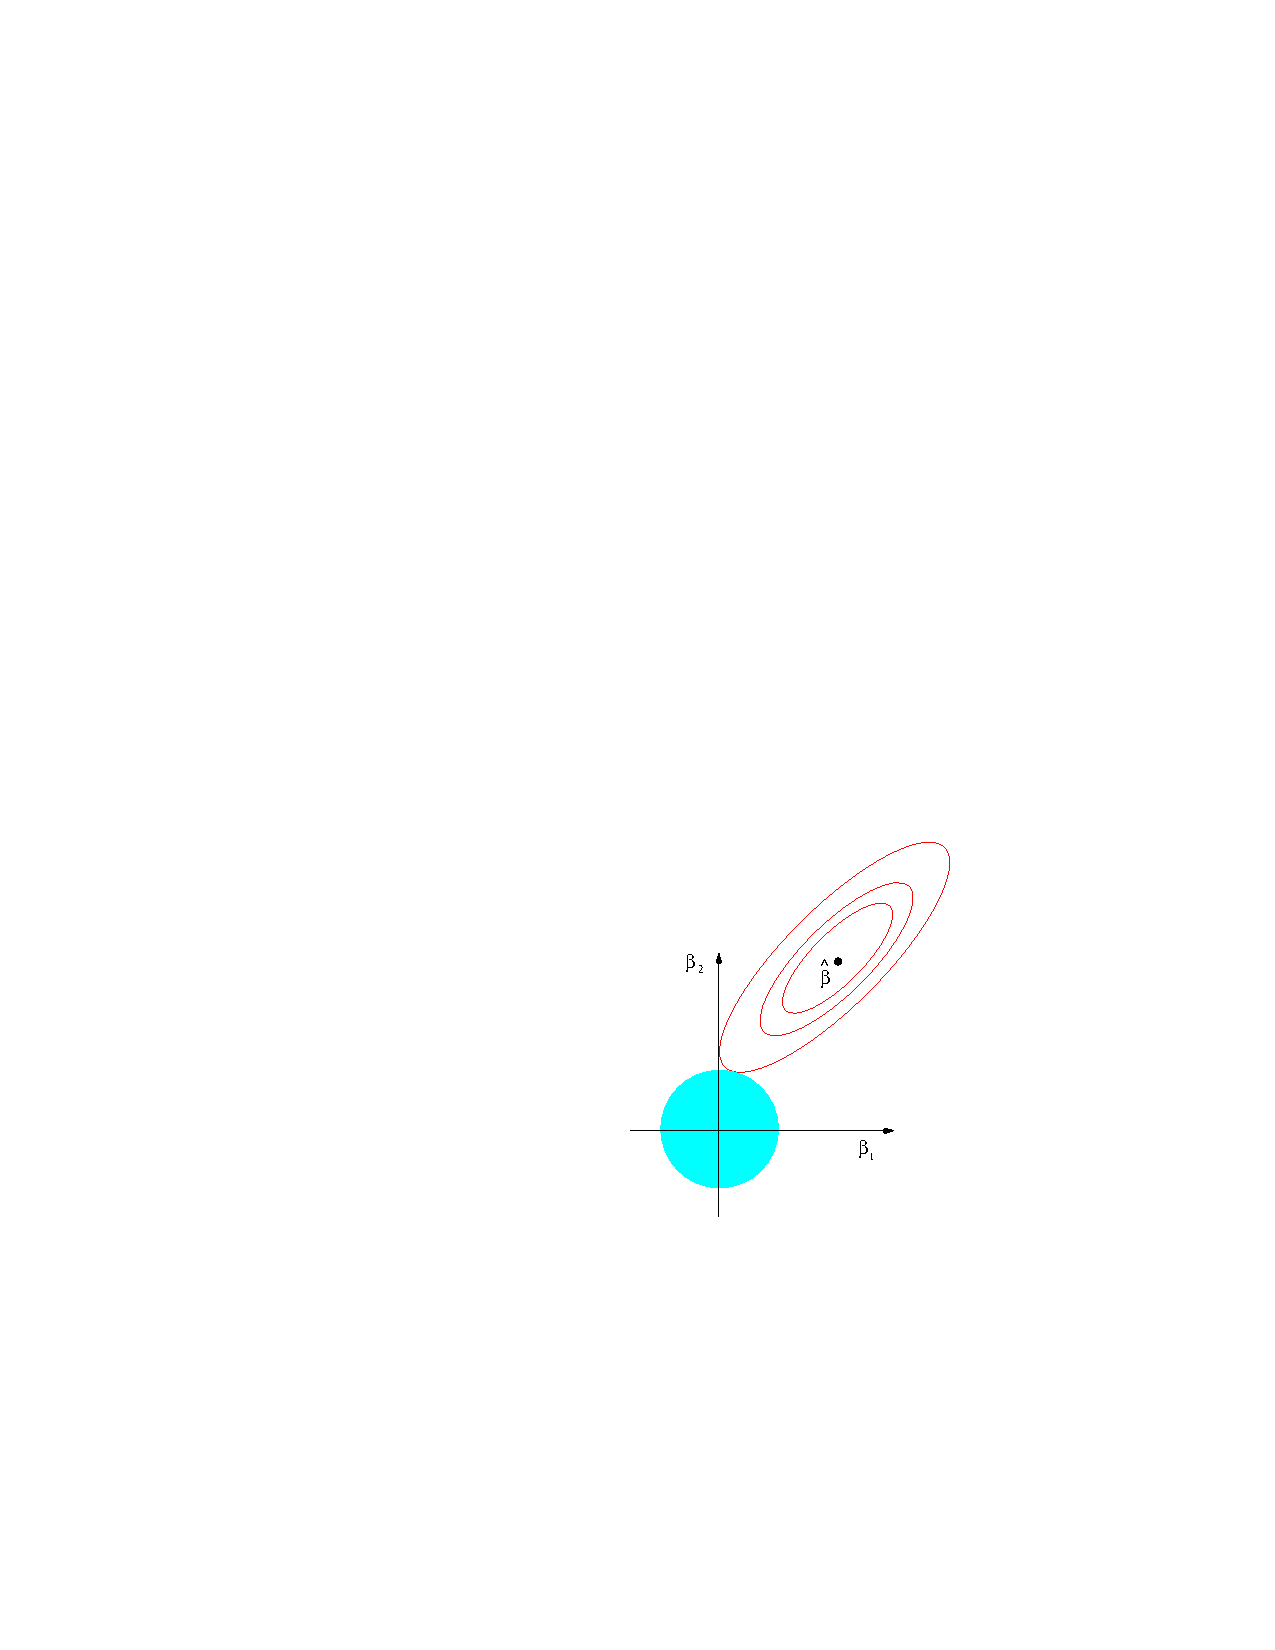
\includegraphics[width=\textwidth]{figures/ml/l2}
  \caption{L2}
  \label{fig:ml:l1l2:L2}
  \end{subfigure}
\caption{
A graphical representation of the L1 and L2 regularization constraints on $\bm{\beta}$ \cite{HastieTF09}.
The best value of $\bm{\beta}$ for optimizing the loss function $L$ is indicated as $\hat{\bm{\beta}}$.
For a given contour in $L$, L1 will tend to force $\bm{\beta}$ along one of the axes,
identically setting some $\beta_{i}$ coefficients to zero,
while L2 is rotationally symmetric and has no such tendencies.
\label{fig:ml:l1l2}
}
\end{figure}

%%%%%%%%%%%%%%%%%%%%%%%%%%%%%%%%%%%%%%%%%%%%%%%%%%%%%%%%
\subsection{L1 -- LASSO}
\label{ml:general:reg:L1}
L1, or LASSO\footnote{Least absolute shrinkage and selection operator.},
regularization uses the norm $\norm{\bm{\beta}}$ \cref{eq:L1}, or taxi cab distance.
As it's geometric constraints on $\bm{\beta}$ are hypercubes,
it tends to set some model parameters to 0, creating sparsity,
and thereby acts as a form of built-in feature selection.

%%%%%%%%%%%%%%%%%%%%%%%%%%%%%%%%%%%%%%%%%%%%%%%%%%%%%%%%
\subsection{L2 -- Ridge}
\label{ml:general:reg:L2}
L2, or ridge, regularization \cref{eq:L2} uses the square of the norm, or euclidean distance.
Models made with L2 regularization are somewhat less interpretable than those made with L1,
as L2 may make many parameters very small, but does not remove them entirely.
The parameters are still shrunk toward zero, and each other,
while highly correlated features are effectively averaged.
L2 is slightly faster to run than L1 computationally as, unlike L1, it
is not represented as a piecewise function and has a closed form expression.

%%%%%%%%%%%%%%%%%%%%%%%%%%%%%%%%%%%%%%%%%%%%%%%%%%%%%%%%
%%%%%%%%%%%%%%%%%%%%%%%%%%%%%%%%%%%%%%%%%%%%%%%%%%%%%%%%
\section{Gradient Descent}
\label{ml:general:grad_descent}
% TODO

%%%%%%%%%%%%%%%%%%%%%%%%%%%%%%%%%%%%%%%%%%%%%%%%%%%%%%%%
\subsection{Stochastic Gradient Descent (SGD)}
\label{ml:general:grad_descent:stochastic}
% TODO

